\documentclass{article}

\usepackage{fancyhdr}
\usepackage{extramarks}
\usepackage{amsmath}
\usepackage{amsthm}
\usepackage{amsfonts}
\usepackage{tikz}
\usepackage{url}
\usepackage[plain]{algorithm}
\usepackage{algpseudocode}
\usepackage{hyperref}
\usetikzlibrary{automata,positioning}

%
% Basic Document Settings
%

\topmargin=-0.45in
\evensidemargin=0in
\oddsidemargin=0in
\textwidth=6.5in
\textheight=9.0in
\headsep=0.25in

\linespread{1.1}

\pagestyle{fancy}
\lhead{\hmwkAuthorName}
\chead{\hmwkClass\ (\hmwkTitle}
\rhead{\firstxmark}
\lfoot{\lastxmark}
\cfoot{\thepage}

\renewcommand\headrulewidth{0.4pt}
\renewcommand\footrulewidth{0.4pt}

\setlength\parindent{0pt}

%
% Create Problem Sections
%

\newcommand{\enterProblemHeader}[1]{
    \nobreak\extramarks{}{Problem \arabic{#1} continued on next page\ldots}\nobreak{}
    \nobreak\extramarks{Problem \arabic{#1} (continued)}{Problem \arabic{#1} continued on next page\ldots}\nobreak{}
}

\newcommand{\exitProblemHeader}[1]{
    \nobreak\extramarks{Problem \arabic{#1} (continued)}{Problem \arabic{#1} continued on next page\ldots}\nobreak{}
    \stepcounter{#1}
    \nobreak\extramarks{Problem \arabic{#1}}{}\nobreak{}
}

\setcounter{secnumdepth}{0}
\newcounter{partCounter}
\newcounter{homeworkProblemCounter}
\setcounter{homeworkProblemCounter}{1}
\nobreak\extramarks{Problem \arabic{homeworkProblemCounter}}{}\nobreak{}

%
% Homework Problem Environment
%
% This environment takes an optional argument. When given, it will adjust the
% problem counter. This is useful for when the problems given for your
% assignment aren't sequential. See the last 3 problems of this template for an
% example.
%
\newenvironment{homeworkProblem}[1][-1]{
    \ifnum#1>0
        \setcounter{homeworkProblemCounter}{#1}
    \fi
    \section{Problem \arabic{homeworkProblemCounter}}
    \setcounter{partCounter}{1}
    \enterProblemHeader{homeworkProblemCounter}
}{
    \exitProblemHeader{homeworkProblemCounter}
}

%
% Homework Details
%   - Title
%   - Due date
%   - Class
%   - Section/Time
%   - Instructor
%   - Author
%

\newcommand{\hmwkTitle}{Homework\ \#2)}
\newcommand{\hmwkDueDate}{\today}
\newcommand{\hmwkClass}{Comp790-Computational Biology}
%\newcommand{\hmwkClassTime}{Section A}
%\newcommand{\hmwkClassInstructor}{Professor Isaac Newton}
\newcommand{\hmwkAuthorName}{\textbf{Your Name Here}} %%modify with your name

%
% Title Page
%

\title{
    \vspace{2in}
    \textmd{\textbf{\hmwkClass\hmwkTitle}}\\
    \normalsize\vspace{0.1in}\small{Due\ on\ \hmwkDueDate\ at 3:10pm}\\
    %$\vspace{0.1in}\large{\textit{\hmwkClassInstructor\ }}
    \vspace{3in}
}

\author{\hmwkAuthorName}
\date{}

\renewcommand{\part}[1]{\textbf{\large Part \Alph{partCounter}}\stepcounter{partCounter}\\}

%
% Various Helper Commands
%

% Useful for algorithms
\newcommand{\alg}[1]{\textsc{\bfseries \footnotesize #1}}

% For derivatives
\newcommand{\deriv}[1]{\frac{\mathrm{d}}{\mathrm{d}x} (#1)}

% For partial derivatives
\newcommand{\pderiv}[2]{\frac{\partial}{\partial #1} (#2)}

% Integral dx
\newcommand{\dx}{\mathrm{d}x}

% Alias for the Solution section header
\newcommand{\solution}{\textbf{\large Solution}}

% Probability commands: Expectation, Variance, Covariance, Bias
\newcommand{\E}{\mathrm{E}}
\newcommand{\Var}{\mathrm{Var}}
\newcommand{\Cov}{\mathrm{Cov}}
\newcommand{\Bias}{\mathrm{Bias}}

\begin{document}

%\maketitle

%\pagebreak
\begin{itemize}
\item This homework is due at 11:59pm on April 21, 2022. Please submit by email to \path{natalies@cs.unc.edu+comp790}. 
\item There are a few files provided:
\begin{itemize}
\item Protein-Protein Interaction Network 1, with edges determined according to co-expression in \path{Coexpress_Edges.csv}
\item Protein-Protein Interaction Network 2, with edges determined according to experimental information given in \path{Experimental_Edges.csv}
\end{itemize}
\item You are welcome to consult with other colleagues, but please write up your own independent solution. 
\item You are welcome to use Python, Julia, or R here.
\item You are welcome to write up your assignment using the \path{HW2_790-166.tex} template, or write up the solutions in the method of your choice. 
\item This homework is worth 62 points total. 
\item Please submit your final writeup as a PDF. Please try not to end me pages of output from Jupyter notebooks :) I simply want to see the few lines of code you used to answer each sub-question.
\item Make sure to comment and elaborate on your answers in places where you are asked to comment! 
\end{itemize}

\begin{homeworkProblem}
{\bf Understanding the Rayleigh Ritz Theorem} (12 points)

Here we will empirically explore the Rayleigh Ritz Theorem which says the following. 

\begin{itemize}
\item Let ${\bf A} \in \mathbb{R}^{N \times N}$ be a square symmetric matrix with eigenvalues $\lambda_{1} \le \lambda_{2} \le \dots \le \lambda_{n}$ and corresponding eigenvectors $\{{\bf v}_{1}, {\bf v}_{2}, \dots {\bf v}_{n}\}$. Defining $R_{\bf A}({\bf x})= \frac{{\bf x}^{T}{\bf A}{\bf x}}{{\bf x}^{T}{\bf x}}$, then the minimum value of $R_{\bf A}({\bf x})$ is $\lambda_{1}$ and occurs when ${\bf x}={\bf v}_{1}$.
\item Obviously, this is a nice property to understand, as ${\bf x}^{T}{\bf A}{\bf x}$ represents the quadratic form that we are often trying to minimize.
\item This property can be extended to find the matrix ${\bf X}$ that minimizes $\text{trace}({\bf X}^{T}{\bf L}{\bf X})$. Specifically, the $k$-dimensional matrix, ${\bf X}$ that minimizes $\text{trace}({\bf X}^{T}{\bf L}{\bf X})$ is the first $k$ eigenvectors of ${\bf L}$ (e.g. those corresponding to the $k$ smallest eigenvalues) and the minimum value obtained for $\text{trace}({\bf X}^{T}{\bf L}{\bf X})$ will be $\lambda_{1}+\lambda_{2}+ \dots + \lambda_{k}.$
\end{itemize}

\end{homeworkProblem}

\begin{figure}[H]
\begin{center}
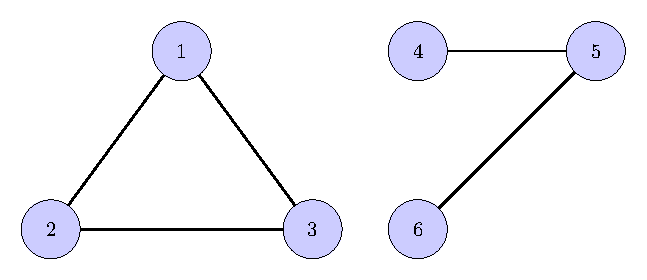
\includegraphics[scale=0.5]{tikz.pdf}
\caption{The graph, $\mathcal{G}$ that we already met in homework 1. }
\end{center}
\end{figure}

\begin{enumerate}
\item {\bf Problem Setup 1} (1 point) Create the adjacency matrix, ${\bf A}$ for $\mathcal{G}$ and compute the graph Laplacian matrix, ${\bf L}$ for this graph. Note that you already did this in homework 1. Just copy it here! 
\item {\bf Problem Setup 2} (1 point) Find the eigenvalues and eigenvectors of ${\bf L}$. Note that you also have done this in homework 1. 
\item {\bf Eigenvalue Sorting} (2 points). We first need to order the eigenvalues of ${\bf L}$ from largest to smallest. That is, you need to return the indices of eigenvalues that would sort them from smallest to largest. 
\item {\bf What Won't Be the Minimum} (2 points). Find the fourth smallest eigenvalue, ${\lambda}_{4}$ and its corresponding eigenvector ${\bf v}_{4}$. Evaluate ${\bf v}_{4}^{T}{\bf L}{\bf v}_{4}$ and write down the number that you get. 
\item {\bf Compare to the Following, which will be smaller} (2 points). Find the first smallest eigenvalue, ${\lambda}_{1}$ and its corresponding eigenvector ${\bf v}_{1}$. Evaluate ${\bf v}_{1}^{T}{\bf L}{\bf v}_{1}$ and write down the number that you get. Comment on this wrt what you got using the fourth eigenvalue/eigenvector. 
\item {\bf Forming the Non-Optimal 2d Embedding} (2 points). Now we will use the eigenvectors that minimize $\text{trace}({\bf X}^{T}{\bf L}{\bf X})$. Form a matrix with two columns where the first column is the third eigenvector ${\bf v}_{3}$ and the second column is the fourth eigenvector ${\bf v}_{4}$. Define the embedding matrix, ${\bf E}$ as the matrix that horizontally concatenates ${\bf v}_{3}$ and ${\bf v}_{4}$ as ${\bf E}=[{\bf v}_{3} | {\bf v}_{4}]$. 
\begin{itemize}
\item Compute $\text{trace}({\bf E}^{T}{\bf L}{\bf E})$. Record what you get.
\item Compute $\lambda_{3}+\lambda_{4}$ and comment about what you get with respect to the trace you just computed. 
\end{itemize}
\item {\bf Forming the Optimal 2 Embedding} (2 points) Now we will use the eigenvectors that minimize $\text{trace}({\bf X}^{T}{\bf L}{\bf X})$. Form a matrix with two columns where the first column is the first eigenvector ${\bf v}_{1}$ and the second column is the second eigenvector ${\bf v}_{2}$. Define the embedding matrix, ${\bf E}$ as the matrix that horizontally concatenates ${\bf v}_{1}$ and ${\bf v}_{2}$ as ${\bf E}=[{\bf v}_{1} | {\bf v}_{2}]$. 
\begin{itemize}
\item Compute $\text{trace}({\bf E}^{T}{\bf L}{\bf E})$. Record what you get.
\item Compute $\lambda_{1}+\lambda_{2}$ and comment about what you get with respect to the trace you just computed. 
\end{itemize}

\end{enumerate}

\begin{homeworkProblem} (50 Points Total)
{\bf Protein-Protein Interaction (PPI) Graph Alignment} \\

Two protein-protein interaction networks for Humans were downloaded from the string database \url{https://string-db.org/} and pre-processed to produce sufficiently large but not too large subgraphs. In the first graph, edges were determined according to co-expression information \path{Coexpress_Edges.csv}. In the second graph, edges were determined according to validated, experimental information. Our challenge is to apply a graph alignment technique to see if the same proteins map to each other between these two graphs. 

Recall REGAL alignment \url{https://arxiv.org/pdf/1802.06257.pdf}. The following homework sub-problems will {\bf walk us through implementing the REGAL graph alignment approach}. \\

1) {\bf Constructing Node Features (5 points):} The first part of REGAL is to create a feature vector for each node that helps to summarize something about its context. We will use a simple $k$-hop method to construct a feature vector for each node. Recall that for a node, $i$, its `$k$-hop subgraph` can be obtained by considering nodes that are within $k$ hops from $i$. (Hint: you may find the following useful \url{https://networkx.org/documentation/stable//reference/generated/networkx.generators.ego.ego_graph.html}). \\

 We will consider $k$-hop networks for $k=1,2,3,4$. {\bf Write a function, where for a particular $k$, you collect the set of neighboring nodes within $k$ hops of each node and summarize the degree distribution of these collective `$k$-hop neighbors` with 4 statistics : \{\text{min degree}, \text{median degree}, \text{mean degree}, \text{max degree}\}.} After doing this for each value of $k$, you should ultimately be able to represent each node with 16 features (4 considered hops $\times$ 4 summary statistics per hop). As an example, assuming Graph 1 has $N_{1}$ nodes, define its node feature matrix, ${\bf X}_{1} \in \mathbb{R}^{N_{1} \times 16}$ matrix. \\

2) {\bf Intuition Building (5 points):} Use your new function to build the described feature vectors for the first graph, \path{Coexpress_Edges.csv} . Assuming this network has $N_{1}$ nodes, {\bf project these $N_{1}$ nodes into two dimensions using your dimensionality reduction method of choice}, based on the 16 computed features (${\bf X}_{1} \in \mathbb{R}^{N_{1} \times 16}$). \\

3) {\bf Choosing Landmarks (5 points):} Recall that REGAL constructs an embedding for each node by specifying landmark nodes that have been collected across both of the graphs being aligned. Choose a set of $d$ landmark nodes {\bf collectively} across Graphs 1 and 2. You can play with $d$ later, but perhaps $d=30$ is a good place to start. You can choose the set of $d$ landmarks at random, or use a more sophisticated approach. {\bf Explain your choice of landmarks and write a function to return these landmark nodes}.  \\

4) {\bf Computing Similarities to Landmarks (5 points):} In part 1), you wrote a function to compute feature vectors for each node. Assuming Graph 1 has $N_{1}$ nodes and Graph 2 has $N_{2}$ nodes, {\bf write a function that computes a similarity measure in this 16-dimensional space between each of the nodes in Graph 1 and Graph 2 to each of the $d$ landmarks.} So, you should en up with a matrix, ${\bf C} \in \mathbb{R}^{(N_{1} + N_{2}) \times d}$. \\

5) {\bf Extract Landmark $\times$ Landmark Matrix (5 points):} As you know, the ${\bf C}$ that you constructed contains the $d$ landmark nodes! Write a function to construct ${\bf W} \in \mathbb{R}^{d \times d}$ submatrix of ${\bf C}$ where the similarities between the landmarks were stored. \\


6) {\bf Embedding via Landmarks (5 points)}: Given Theorem 3.1 in \url{https://arxiv.org/pdf/1802.06257.pdf},  we can compute the collective node embedding matrix (across Network 1 and Network 2), $\tilde{\bf Y} \in \mathbb{R}^{(N_{1} + N_{2}) \times d}$, as

$$\tilde{\bf Y}={\bf C}{\bf U}{\boldsymbol \Sigma}^{1/2}$$. 

Recall that here, ${\bf U}$ and ${\boldsymbol \Sigma}$ are obtained through an SVD on the pseudo inverse (${\bf W}^{\text{pinv}}$) of the (landmark $\times$ landmark) similarity matrix, ${\bf W} \in \mathbb{R}^{d \times d}$ extracted from ${\bf C}$.

 $${\bf W}^{\text{pinv}}={\bf U}{\boldsymbol \Sigma}{\bf V}^{T}$$

Hints: These are useful for pseudoinverse (\url{https://numpy.org/doc/stable/reference/generated/numpy.linalg.pinv.html}) and SVD (\url{https://numpy.org/doc/stable/reference/generated/numpy.linalg.svd.html}). \\

{\bf Given this information, write a function to compute $\tilde{\bf Y}$.} \\

7) {\bf Putting it All Together Visualization 1 (5 points):} You have now defined an embedding for all nodes in Networks 1 and 2 in some $d$-dimensional space through $\tilde{\bf Y}$. {\bf Use your favorite dimensionality reduction method of choice to project the collective set of nodes in Networks 1 and 2 into two dimensions. Color the nodes by which network they are from. Comment on any observations.} \\

8) {\bf Alignment Between Graphs (5 points):} Given $\tilde{\bf Y}$, {\bf calculate a similarity score (your choice) between each node in Network 1 and every node in Network 2.}  \\

9) {\bf Creativity (5 points):} Now that you have the entire pipeline in place, play around with it a bit. For example, considering changing how you define the features for nodes in part 1), changing the value of $d$, changing how you choose landmarks, or anything else that is interesting to you! {\bf Re-run steps 1-7 with your modification and comment on how it changes the interpretation of alignment between Network 1 and Network 2 given in $\tilde{\bf Y}$}. \\

10) {\bf Creativity Part 2 (5 points):} Imagine a collaborator dropped these two networks on your desk. They are paying you from their grant, so you need to produce something to give them. {\bf Create a visualization of your choice that reflects something about the similarity between Network 1 and Network 2} (in terms of node alignment, clustering structure, etc). \\

{\bf Congratulations! You implemented REGAL from scratch!}



\end{homeworkProblem}

\end{document}